% !TeX spellcheck = en_US
% !TeX encoding = utf8
% !TeX program = xelatex
% !BIB program = bibtex
% !TeX spellcheck = en_US
% !TeX encoding = utf8
% !TeX program = xelatex
% !BIB program = bibtex

\documentclass[12pt]{article}
	\usepackage{amsmath,amssymb,amsfonts}
	\usepackage{latexsym}
	\usepackage{graphicx}
	\usepackage{verbatim}
	\usepackage{booktabs}
	\usepackage[usenames,dvipsnames,svgnames,table]{xcolor}
	\usepackage{todonotes} % Required for the boxes that questions appear in
	\usepackage{mmstyles}
	% \newcommand{\mybox}[1]
	% {
	% \par\noindent
	% \todo[inline, backgroundcolor=SkyBlue!40,bordercolor=SkyBlue,size=\large]{\textbf{#1}}
	% }

	\usepackage[top=25mm, bottom=25mm, left=18mm, right=18mm]{geometry}

	\usepackage{fancyhdr}
	\pagestyle{fancy}
	\lhead{Linear Optimization Prj \#1}
	\chead{}
	\rhead{Due: May 4, 23:59:59}
	\renewcommand{\headrulewidth}{0.3pt}
	\usepackage[backend=biber]{biblatex} 
	\bibliography{ref.bib}
	\addbibresource{ref.bib}
	\usepackage{listings}
	\title{\textbf{Linear Optimization Prj \#1}}
	\author{Due: May 4, 23:59:59}
	\date{}

	\usepackage{multirow}

	\newcommand{\abs}[1]{\left| #1 \right| }
	\newcommand{\norm}[1]{\left\| {#1} \right\|}
	\newcommand{\red}[1]{{\color{red}{#1}}}
	\usepackage{titlesec,titletoc} 
	\renewcommand*{\thesection}{\color{NavyBlue} \arabic{section} } 
	\renewcommand*{\thesubsection}{\color{SkyBlue} \arabic{section} }
	\titleformat{\section}[hang]{\bfseries}{\thesection}{1em}{}{}
	\titleformat{\subsection}[hang]{\itshape}{\thesubsection}{1em}{}{}
	
	% \setlength{\parsep}{0em}
	% \setlength{\itemsep}{0pt}
	\setlength{\parskip}{.33em}
	\setlength{\parindent}{0em}	

	\providecommand{\tightlist}{%
	\setlength{\itemsep}{0pt}\setlength{\parskip}{0pt}}
  
\begin{document}
% \vspace{-1em}
\maketitle

\textbf{\color{NavyBlue}Instruction:} Write a report and complete code. Download the code from ftp (10.13.71.168). Upload
report and code to ftp (10.13.72.84) or send email to 907682447@qq.com.
\begin{itemize}
	\tightlist
	\item The same naming rule as homework2, i.e., prj1\_31xxx.pdf, prj1\_31xxx.zip or rar.
    \item May 5 is the day for exam, please upload project before exam
	\item Upload:
	      \begin{itemize}
		      \tightlist
		      \item    Address: 10.13.72.84
		      \item Username: opt; Passwd:  opt18; Port: 21
	      \end{itemize}
	\item Download:
	      \begin{itemize}
		      \tightlist
		      \item Address: 10.13.71.168
		      \item  Username: opt; Passwd:  opt18; Port: 21
	      \end{itemize}
\end{itemize}

\section{Abstract} 
Machine learning algorithms are increasingly being applied in security-related tasks such as spam and
malware detection, although their security properties against deliberate attacks have not yet been
widely understood. Intelligent and adaptive attackers may indeed exploit specific vulnerabilities
exposed by machine learning techniques to violate system security. Being robust to adversarial
data manipulation is thus an important, additional requirement for machine learning algorithms to
successfully operate in adversarial settings. In this project, we will reproduce paper \cite{biggio2011support}. 

\section{Basic}
\begin{itemize}
    \item Read paper \cite{biggio2011support}. For adversarial label flips, we can further ref. to \cite{xiao2015support}. Read code, ‘main.py’,
    ‘data.py’ and ‘svm.py’. The code is developed under python3.6 and partially tested under
    python2.7, i.e.,the code are supposed to be compatible with both environments.
    \item Install ’cvxopt’ via conda or pip. Run ‘main.py’ with exp=’toy’ and kernel=’linear’. We may
    see something like fig \ref{fig:linear}. 
    % Run ‘main.py’ with exp=’toy’ and kernel=’rbf’, the potential results are shown in fig \ref{fig:rbf}.

    \begin{figure}
        \centering 
        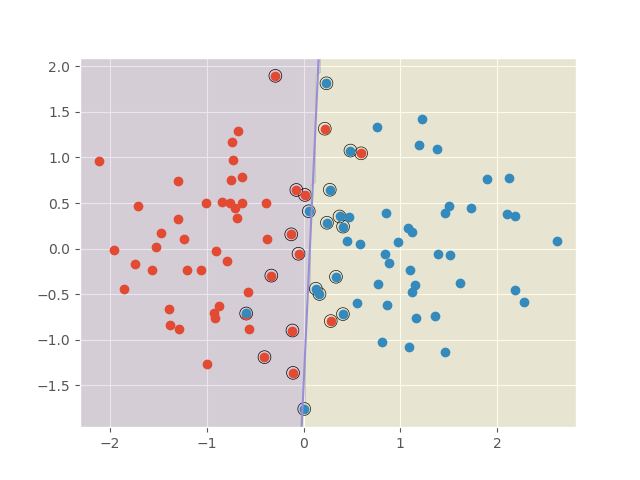
\includegraphics[width=.45\textwidth]{./fig/linear/ori.png} 
        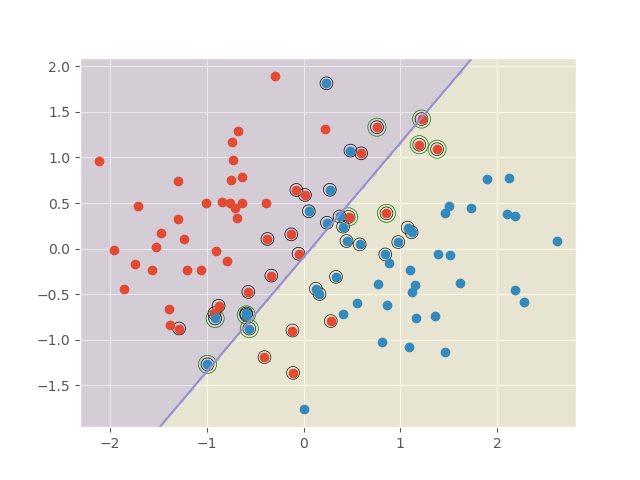
\includegraphics[width=.45\textwidth]{./fig/linear/ln.png} \\
        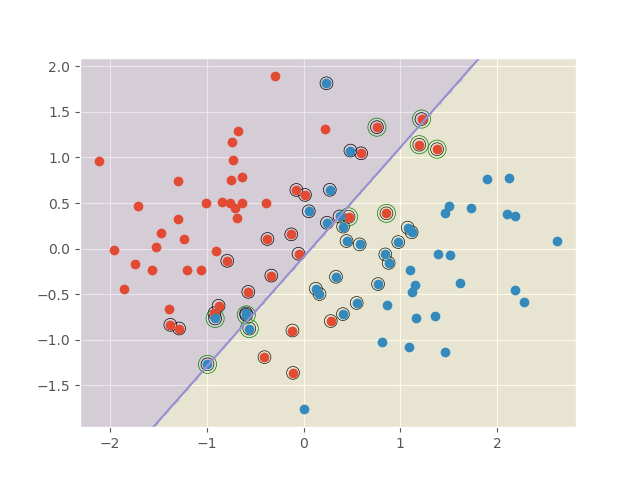
\includegraphics[width=.45\textwidth]{./fig/linear/ln.robust.mu.0.1.png} 
        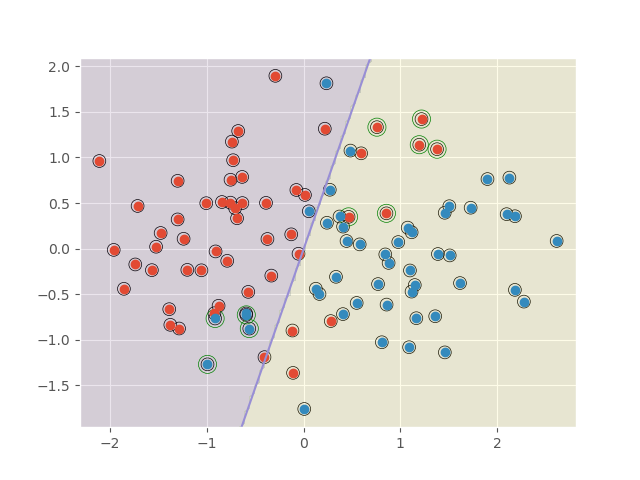
\includegraphics[width=.45\textwidth]{./fig/linear/ln.robust.mu.0.5.png} 
        \caption{ Results with linear kernel. \textbf{TopLeft}: Train on untainted data. \textbf{TR}: Train on tainted data.
        \textbf{BL}: Train LN-robust SVM on tainted data with $\mu  = 0.1$. \textbf{BR}: with $\mu = 0.5$.}
        \label{fig:linear}
    \end{figure}

    When seed=16, the toy data are exactly the same. However, the adversarial label flips process
    can be different. We observe different separating hyperplane in each running, but there exists
    some pattern and conclusion in the results. Show them. We may ref. to section 5 in paper \cite{biggio2011support}.
    \item  Run ‘main.py’ with exp=’sonar’ and plot something like fig \ref{fig:sec6}, which corresponding to section 6 in paper \cite{biggio2011support} 

    \begin{figure}
        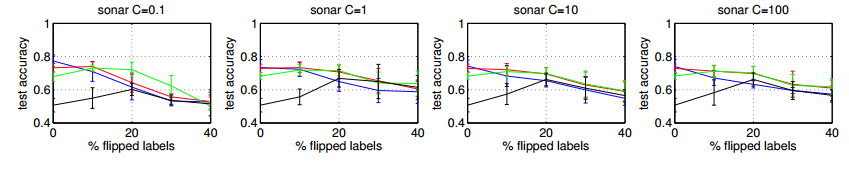
\includegraphics[width=.9\textwidth]{fig/sec6.png} 
        \caption{Test accuracy w.r.t. flipped ratio, C, and different model} 
        \label{fig:sec6}
    \end{figure}
    \item Run ‘main.py’ with exp=’proc’ and improve the algorithm and run again. There are many
    algorithms to choose, e.g., following the paper, try other machine learning method like logistic
    regression and use the method mentioned on the class, i.e., train a model, observe the statistic
    of dataset and clean outlier, and training and observe ...

    Remember to include the results ‘y-pred’ in zip. We will evaluate our results with the metric
    of accuracy and become part of our grading. We are allowed to upload less and equal than
    5 results naming by ‘y-pred.*’, e.g., ‘y-predblabla’, ‘y-pred.315xx’, ‘y-pred.assume.adversarial’
    and so on. We take the maximum accuracy. And the format of ‘y-pred.*’ file are supposed
    to be the same as what generated by ‘main.py’ with exp=’proc’, i.e., do not modify read and
    write code in ‘main.py’.

    About the information of the dataset, we can say: (1). training data is polluted by label flip
    noise and no other noise. (2). label flip is either random flip or adversarial (to svm model) flip.
    (3). Flip ratio is around 20\%. (4). Testing data is not polluted by any noise.
    
    We are allowed to use other packages or frameworks, not strictly limited to the framework provided by TA. 
    \item Last but not the least, we'd better cover these points in a \textbf{fluent} report. 
\end{itemize}

\section{Bonus}

\begin{itemize}    
    \item Try other hyperparameter in former experiments. Analyze and illustrate the results with figures and tables. 
    \item Translate one or more parts in paper \cite{biggio2011support}, \eg, section of introduction, related work, ,algorithms and experiments. 
    \item Read, comment the code, and explain the procedure of training SVM and adding label flip noise in the report. 
    \item Understanding adversarial label flip attack algorithm: What is the range of $(\alpha,b)$ and $(\alpha^{rnd},b^{rnd})$, \ie, min and max value. Explain $v_i \leftarrow \alpha_i /C -\beta_1 s_i -\beta_2 q_i $. Discuss the idea of label flip attack algorithm. 
    \item Any novel ideas and open questions. 
\end{itemize}
\printbibliography
\end{document}

